\section{A neural network for content popularity prediction} \label{neural_network}

\subsection{Fully connected feedforward neural networks} \label{feedforward_nn}

\begin{figure}[b!]
	\centering
	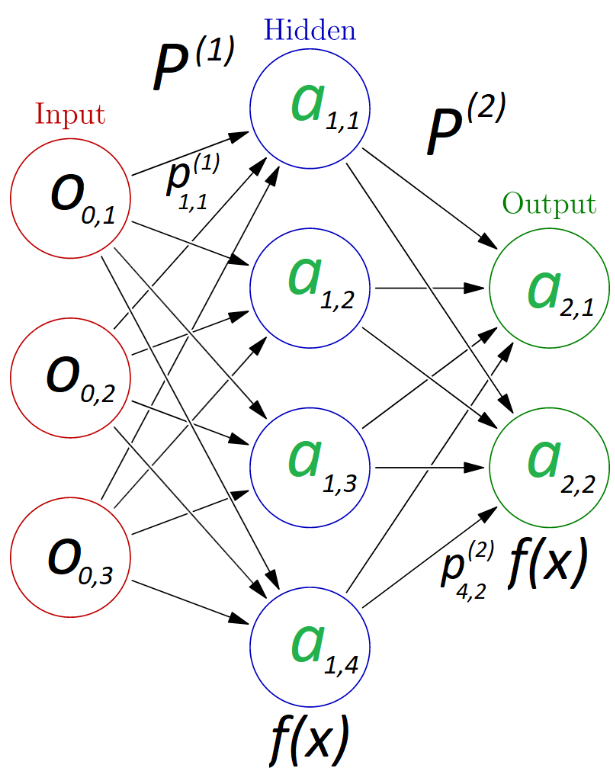
\includegraphics[totalheight=7cm]{pics/nn_1.png}
	\caption{Fully connected feedforward network.}
	\label{fig:nn1}
\end{figure}

The simplest example of a neural network is a fully connected feedforward neural network. The smallest block of a neural network is a neuron. A neuron sums all of its inputs and produces one output. Neurons are stacked into layers. The output of the layer is a column vector consisting of the outputs of all of the layer's neurons. Let's denote the output of the layer $L$ as $o_L$. In a fully connected feedforward neural network all of the neurons in a layer are connected with all of the neurons in the next layer. Each connection has a weight. Weights between layers $ L - 1 $ and $ L  $ form a matrix $ P^L $, where $ p^{L}_{i,j}$ is the weight of connection between $i$-th neuron  of layer $L - 1$ and $j$-th neuron of layer $L$. Following this notation, we can define the output $o_L$ of the layer $L$ as $o_L = o^{\intercal}_{(L-1)} P^L$.

Each layer can also have an activation function $ f(x) $. Activation of the layer $ L $ is the $ a_L = f(o_L) $. Typical activation functions used are:

\vspace{4pt}
Sigmoid: $ f(x) $ \Large $ = \frac{1}{(1 + e^{-x})} $.
\normalsize

\vspace{4pt}
Rectified Linear Unit: $ f(x) = max(0, x) $.

Hyperbolic Tangent: $ f(x) $ \Large $ = \frac{sinh(x)}{cosh(x)} = \frac{e^x - e^{-x}}{e^x + e^{-x}}$.
\normalsize
\vspace{4pt}

The introduction of the activation functions ads nonlinearity to the input propagation through the neural network which should positively influence the accuracy of predictions.

It is a common practice to add a bias neuron to layers of a neural network. A bias neuron always outputs 1 and is intended to improve the accuracy by allowing to shift the output of any layer in any dimension.

To train the neural network a dataset is required. Each row of the dataset contains the input of the neural network and true output. Forwarding the input through the network provides the output which then can be used to calculate the error, or loss, using the true output from the dataset and the provided loss function, but only for the output layer. The error on the output layer can be used to calculate the error on previous layers in a process called error backpropagation \cite{13}. The error on each layer is used to update the weights through gradient descent. Even though many loss functions to calculate the error have been proposed, we are going to apply classical loss function - Mean Squared Error (MSE):

%\Large
$$ g(x) = \frac{\sum_{i=1}^{N} (y_{true} - y_{pred})^2}{N} $$
%\normalsize

\subsection{Chosen architecture} \label{chosen_architecture}

There are a few degrees of freedom in neural network usage. The first one is the number of layers. Adding more layers allows learning more complex relations but decreases the performance and requires more learning iterations. The second degree of freedom is the number of neurons in each layer, but usually is limited only to internal layers since the number of neurons in input and output layers is determined by the dimension of input and output data. The tradeoffs are the same as with the number of layers. There are no clear rules or recommendations on the topic of selection of activation functions, we will stick to established well-performing options.

We aim to use a neural network to predict the future popularity of objects based on, mainly, the in past popularity. To extract the data from the request traces and form a dataset for neural network consumption, it is possible to split the request trace in time frames (or time windows) and calculate the popularity of each item in each time frame. Let us denote this popularity as $ X_{i,j} $. Each row would consist of $ K + 1 $ popularities values, K values are input, and 1 is the output. To keep popularity independent of the number of requests in the time frame, the popularity of content is represented as the fraction of requests for that content. Using unchanged popularity values as the input of the neural network led to poor performance since the large difference of popularity values, spanning many orders of magnitude, caused the neural network to learn to make good predictions for the most popular objects sacrificing the prediction accuracy for less popular objects. To fix this issue, we decided to apply a transformation for both input and output popularity values. All of the values are transformed by the next formula: $ f(p) = -\log(p + const) $. This transformation reduces the difference between the smallest and the largest values processed by the neural network and improved the accuracy of predictions greatly.

After some consideration, the next neural network architecture has been chosen. We use 4 neurons in the input layer, i.e. we are going to predict the popularity in the future based on popularity in 4 previous time frames with the size of $10^7$ seconds. We will further experiment with both these values discussing the performance of the proposed caching policy. Then the input is feedforwarded through 2 hidden layers with 128 neurons in each. We want to predict the popularity in the next time frame, thus the network has only one neuron in the output layer. To every layer except the output, a bias neuron is added. As for the activation, we concluded that rectified linear unit performs the best. To overcome the "dying ReLU"\cite{14} problem, a variation of ReLU is applied i.e. Leaky ReLU:

$$ f(x) = 
	\begin{cases}
	x, & \text{if } x \geq 0; \\
	a*x,\, 0 < a \ll 1 & \text{otherwise.}
	\end{cases}
$$

\subsection{Performance evaluation} \label{performance_eval}

Continuing with neural networks, we need to determine 1) a way to evaluate the state of neural networks, i.e. to check that network has finished training, and 2) to verify that the predictions made by the network are close to desirable. To deal with the first issue, we can observe the behavior of the value of the loss function through iterations. If the value of the loss function is decreasing with each iteration, then the neural network still hasn't finished training. Otherwise, if the loss is stable through iterations, the training is completed. The second issue can also be addressed by observing the value of the loss function. The loss should converge to a small value. But also we can directly check the predictions made by the neural network by plotting the predictions and true output and visually evaluating the quality of predictions.

Finally, to verify that the neural network is good at generalizing the underlying dependency between the input and the output and not just learned to map input-output pairs for the training dataset, what is called overfitting \cite{15}, we use a separate dataset to evaluate the prediction quality, called the ``validation dataset''. If the loss on the training data is low but high on the validation data, it means that the neural network is overfitted and some actions are required to overcome this issue.

\subsection{Experimental results} \label{experiments_results}

\begin{figure}[b!]
	\centering
	\begin{subfigure}[b]{0.49\linewidth}
		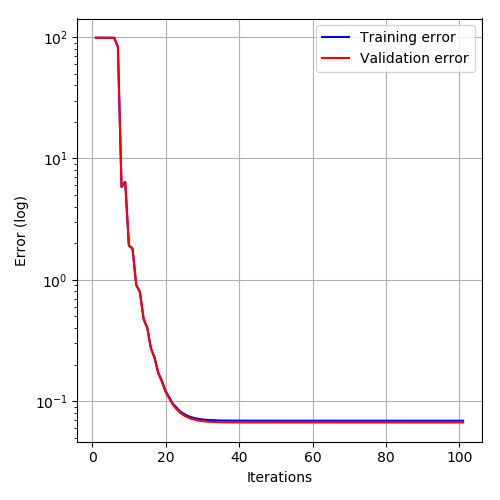
\includegraphics[width=\linewidth]{pics/case1_err.png}
		\caption{Synthetic trace. Case 1.}
	\end{subfigure}
	\begin{subfigure}[b]{0.49\linewidth}
		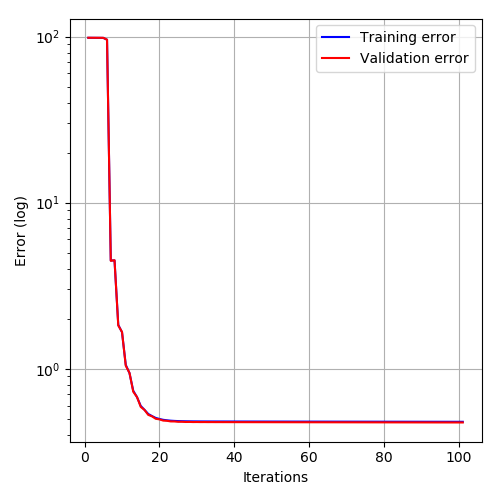
\includegraphics[width=\linewidth]{pics/case2_err.png}
		\caption{Synthetic trace. Case 2.}
	\end{subfigure}
	\caption{Evolution of mean squared error through training iterations.}
	\label{fig:nn3}
\end{figure}

After generating the two synthetic traces with $ 10000 $ unique items in both types, with static and nonstatic popularity as described in Section \ref{synthetic_data}, $ 0.8 $ Zipf's distribution parameter, $ 20 $ milliseconds mean time between requests, and $ 10^7 $ total requests, we evaluated the performance of the proposed architecture of the neural network. To prepare the data from traces for neural network consumption after the generation of the traces was finished, we generated datasets using a size of the window $ 10^7 $ milliseconds. After splitting the datasets into training and validation sets both training and validation loss values converged to small numbers, as you can observe in the Figure \ref{fig:nn3}, which meant that the training is over. In Figure \ref{fig:nn2} you can see what prediction neural networks learned to make in both cases of the synthetic traces. Top plots show how the actual ranking of the items according to their popularity compares with the predicted ranking. In the ideal case, values on the x-axis should be equal to values on the y-axis. Bottom plots show how the actual predicted popularity values compare to real popularity values. Blue dots, which represent predicted values, closely follow red dots, which are real popularity values. From this, we can conclude that this architecture of the neural network is suitable for object popularity prediction.

\begin{figure}[t!]
	\centering
	\begin{subfigure}[b]{0.49\linewidth}
		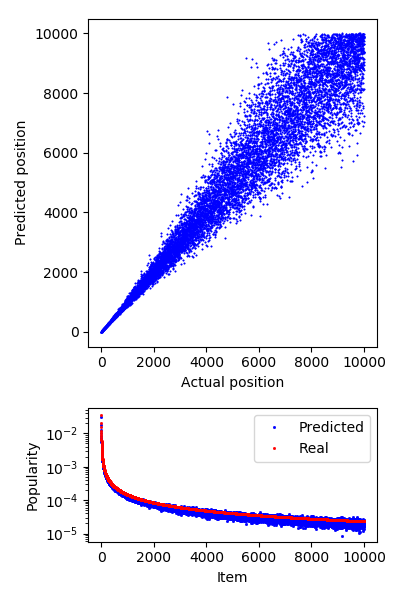
\includegraphics[width=\linewidth]{pics/case1_op.png}
		\caption{Synthetic trace. Case 1.}
	\end{subfigure}
	\begin{subfigure}[b]{0.49\linewidth}
		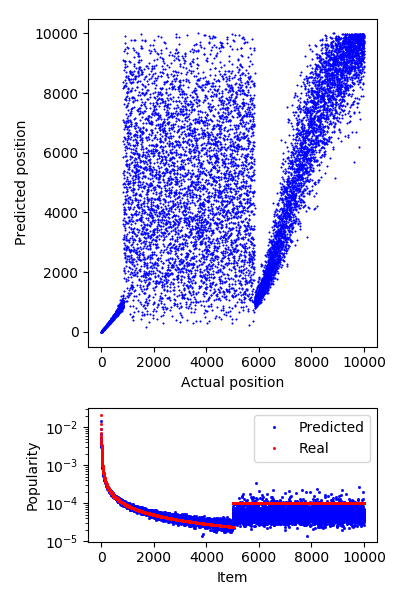
\includegraphics[width=\linewidth]{pics/case2_op.png}
		\caption{Synthetic trace. Case 2.}
	\end{subfigure}
	\caption{Evaluation of neural network prediction quality.}
	\label{fig:nn2}
\end{figure}

\subsection{Adaptation for online scenario} \label{nn_online}

Following the success in the application of a neural network for object popularity predictions, we need to adapt the architecture of the network so it is usable in the online setting, thus the architecture of the neural network is slightly different from the one described in the previous section. In the Figure \ref{fig:cache1} you can see the proposed usage of the neural network by the policy.

\begin{figure}[h!]
	\centering
	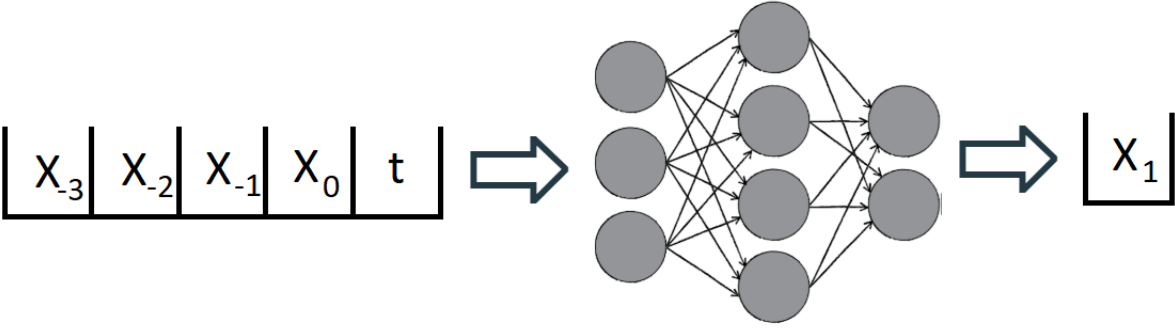
\includegraphics[width=\linewidth]{pics/cache1.png}
	\caption{Neural network architecture for caching policy.}
	\label{fig:cache1}
\end{figure}

\begin{itemize}
	\item $X_{-3}$ through $X_{-1}$ are popularities of the object in the previous 3 time frames;
	\item $X_0$ is the popularity of the object in the current time frame;
	\item $t$ is the fraction of the current time window that has already passed;
	\item $X_1$ is the popularity of the object in the future;
\end{itemize}

The difference is caused by the nature of the application of caching policies. The policy is working in the real-time thus we cannot operate in the framework of only previous and next time frames. $X_0$ represents the popularity in the current time frame. But at the beginning of the time frame, the quality of the value $X_0$ may be low since there will not be enough requests in the time window to estimate the popularity with reasonable accuracy. To help with this issue, we decided to add the parameter $t$. Using this parameter, the neural network will be able to learn to judge the quality of the parameter $X_0$ and make better predictions. Further, we will also experiment with different number of prediction windows and trying to add other metadata to improve the accuracy of predictions.

Next, we are going to introduce a caching policy which relies on neural network presented here to make caching decisions.

